% Chapter 3

\chapter{Results and conclusion} % Write in your own chapter title
\label{Chapter3}

We observe that with our implementation, code is able to detect a moving
person after it's 3 steps move. Figure  \ref{pipeline_images} shows
output images at different stages of pipeline.

\begin{figure}[!b]
\centering
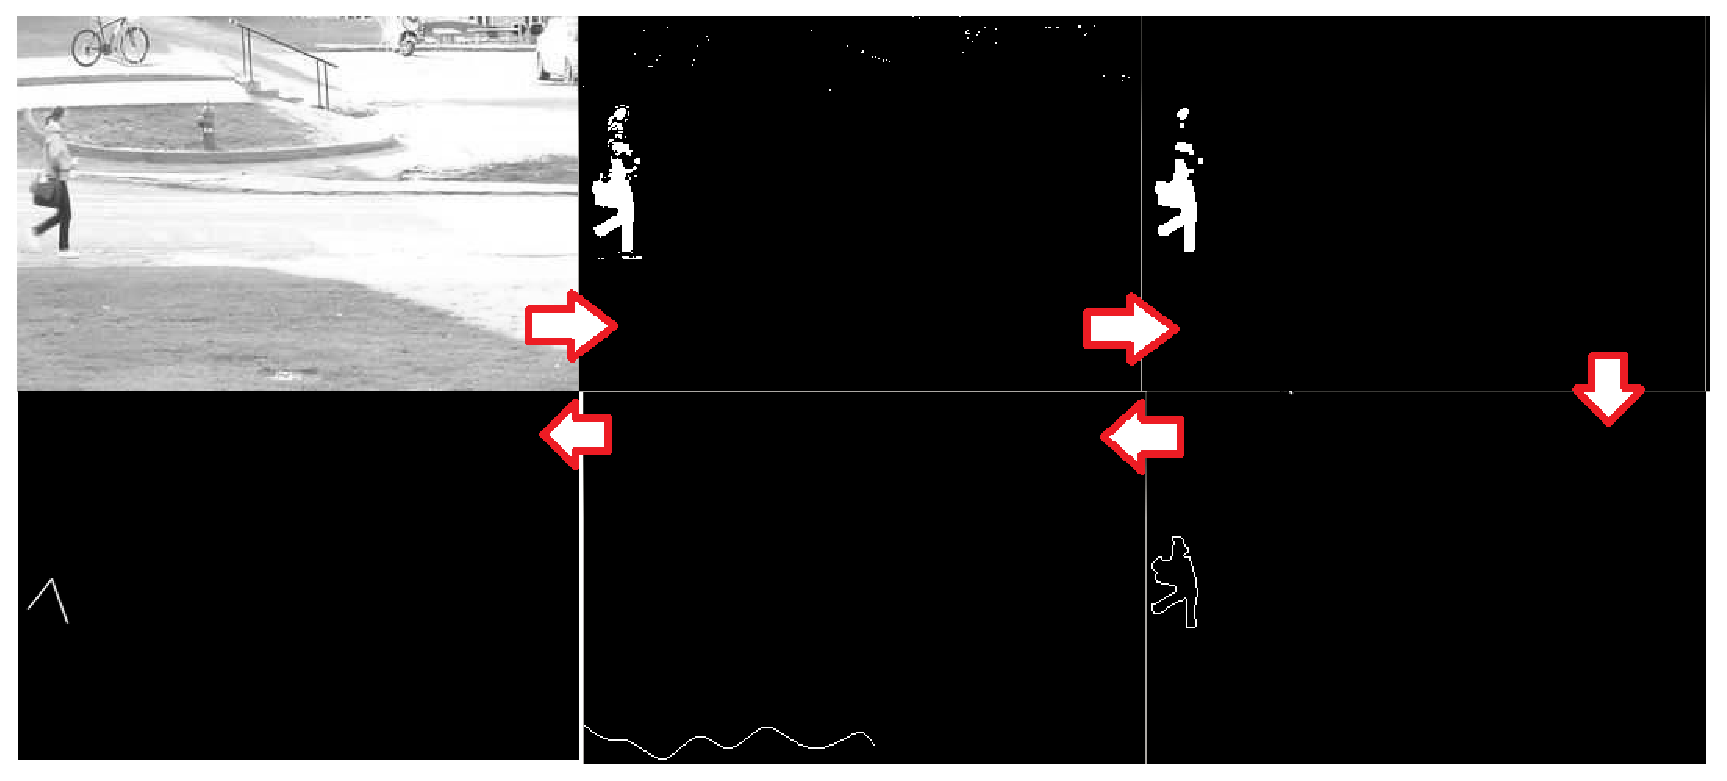
\includegraphics[scale=0.60]{Figures/pipeline_images}
\caption{Images at different stage of pipeline. (From top left in
clockwise order) \textbf{a.} Gray Scale input frame to pipeline
\textbf{b.}Foreground extracted image using Vibe \textbf{c.} Cleaned
image \textbf{d.} Contour of moving object \textbf{e.} Plot of 3 points
of interest, centroid and two distance peaks nearer to bottom left and
bottom right corner of bounding box \textbf{f.} Virtual representation
of scene} 
\label{pipeline_images}
\end{figure}

We have also done experiments with negative images like a person moving
on bicycle, or a vehicle moving on road. Our algorithm is successfully
able to reject these objects. Figure \ref{negative_inputs} shows that
how does this implementation rejects moving vehicle and bicycle and  does
not recognize them as human.
\begin{figure}[!b]
\centering
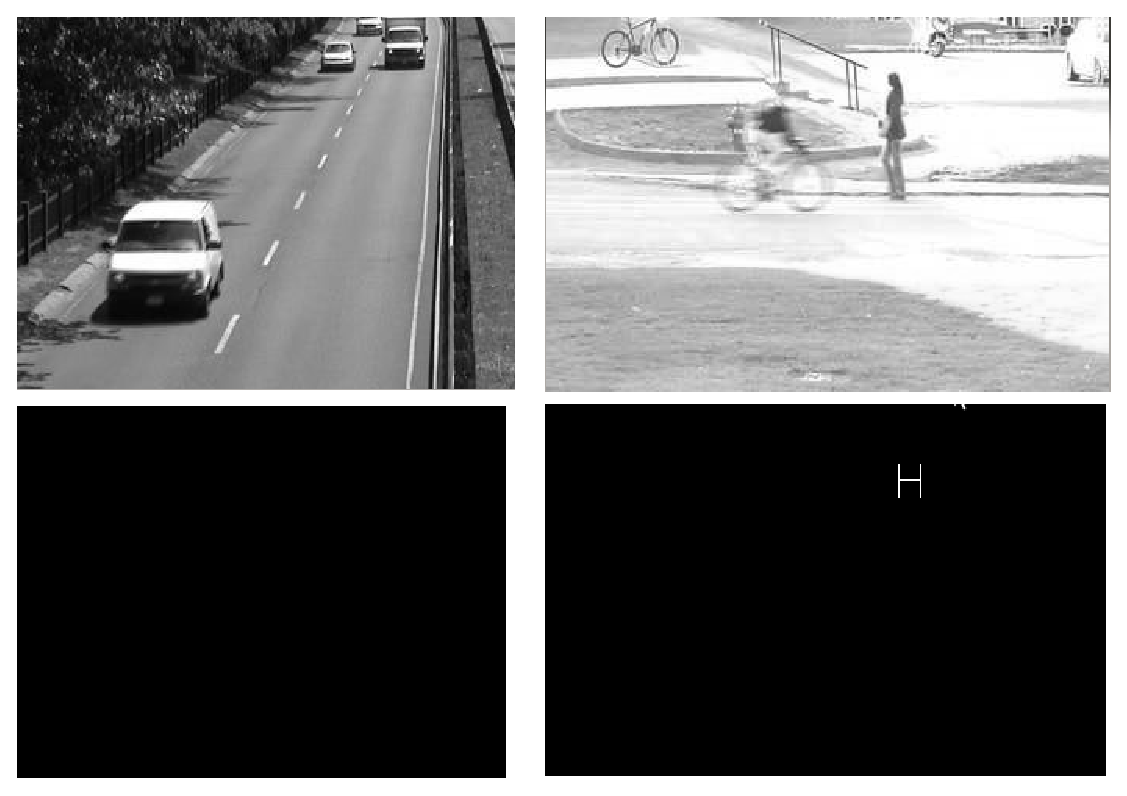
\includegraphics[scale=0.60]{Figures/negative_inputs}
\caption{Input and output of pipeline in case of negative images}
\label{negative_inputs}
\end{figure}


Comparison of proposed framework with HAAR and IDIAP detection algorithm
in figure \ref{pipeline_execution_time} shows that, this is quite
faster. Our pipeline takes just 3.6 mS on the average, while HARR and
IDIAP takes around 20mS and 248 mS respectively per frame. This timing
was observed with a system having DMIPS = 800.

\begin{figure}[!b]
\centering
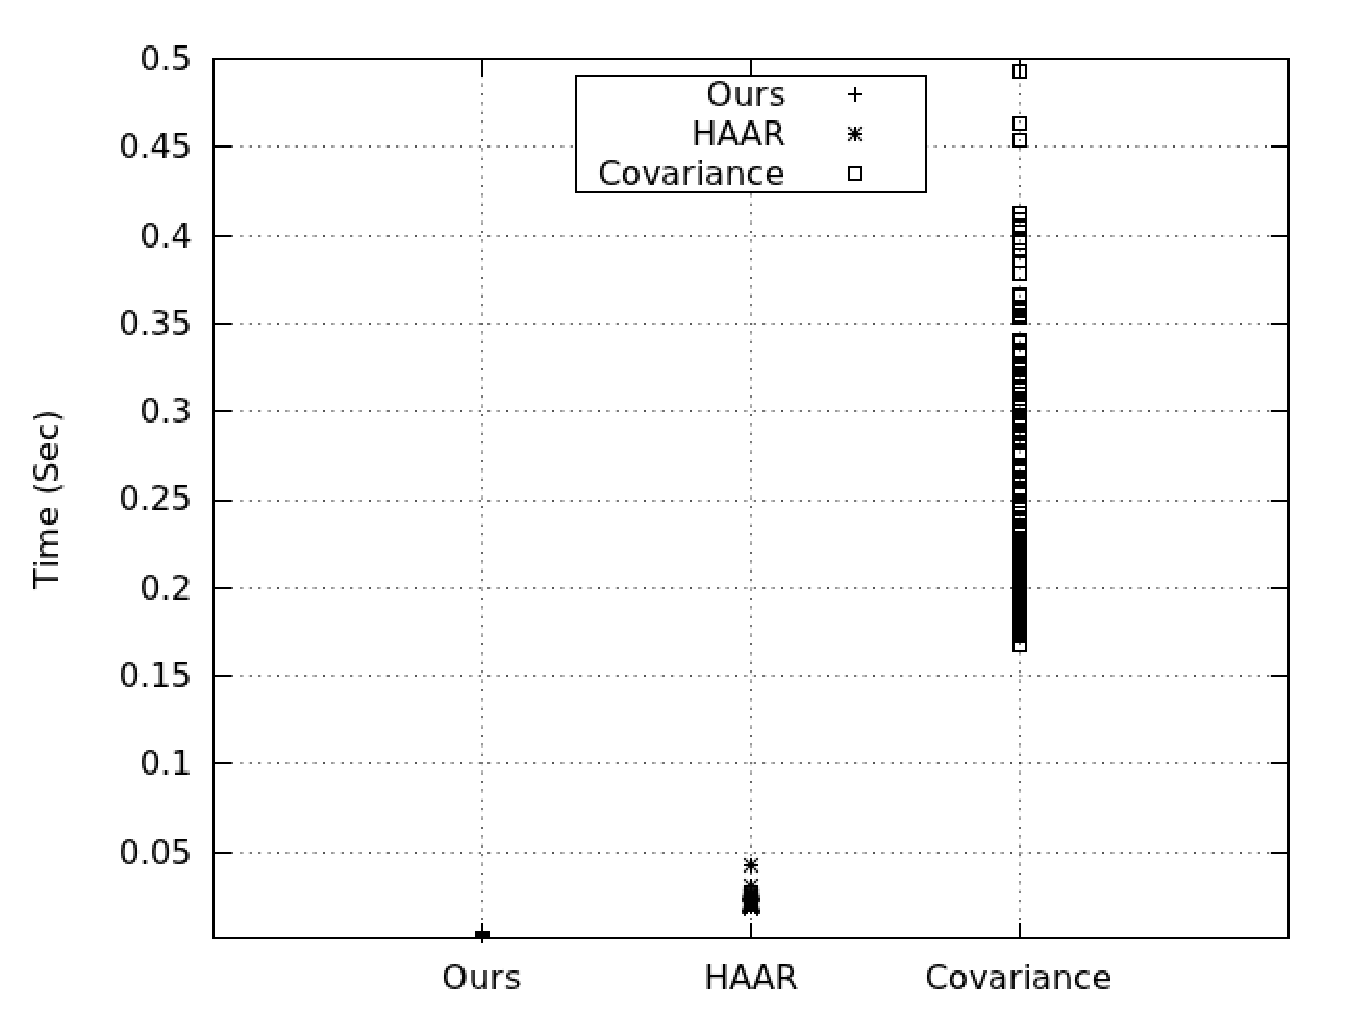
\includegraphics[scale=0.60]{Figures/pipeline_execution_time}
\caption{Variation of different pipeline execution time with a system
having DMIPS=800}
\label{pipeline_execution_time}
\end{figure}

So if a surveillance application requires to identify moving person,
then we might not need to use complex algorithm. Processor like Coretx
M3/M4 are used in an embedded environment with a low power application.
Such processors have DMIPS of 1.25 dmips/Mhz. If we use such processors
at 300 MHz, our pipeline will be able to process one frame in less than
8 mS, and therefore system can go in sleep mode for longer time and
hence can save a lot of powers.


